\documentclass[11pt,aspectratio=169]{beamer}

\usepackage{booktabs}
\usepackage{array}
\usepackage{tikz}
\usetikzlibrary{arrows.meta,positioning,calc,shapes.geometric}
\usepackage{xcolor}
\usepackage{amsmath}

\usetheme[titleformat=smallcaps,progressbar=frametitle]{metropolis}
\definecolor{UTburnt}{HTML}{BF5700}
\definecolor{LBJnavy}{HTML}{172A46}
\definecolor{softgray}{HTML}{F2F3F5}
\definecolor{midgray}{HTML}{6B7280}
\definecolor{goodgreen}{HTML}{2E7D62}
\setbeamercolor{alerted text}{fg=UTburnt}
\setbeamercolor{frametitle}{bg=LBJnavy,fg=white}
\setbeamercolor{progress bar}{fg=UTburnt,bg=gray!25}
\setbeamercolor{block title}{bg=LBJnavy!10,fg=LBJnavy}
\setbeamercolor{block body}{bg=softgray}
\setbeamertemplate{itemize item}{\color{UTburnt}$\blacktriangleright$}
\setbeamertemplate{itemize subitem}{\color{UTburnt}$\bullet$}

\author{Sergio I. Garc\'ia-R\'ios}
\title{From Questions to Data}
\subtitle{Measurement and Exploratory Data Analysis}
\institute{PA 311N: Data Analysis for Public Policy\\LBJ School of Public Affairs}
\date{Fall 2026}

\newcommand{\bigquestion}[1]{%
\begin{center}
\begin{minipage}{0.88\textwidth}
\centering
\Large\color{LBJnavy}\textbf{#1}
\end{minipage}
\end{center}}

\begin{document}

\maketitle

% 2
\begin{frame}{What are we trying to do?}
\large
Public-policy decisions are often arguments about \alert{evidence}.

\vspace{0.7em}
\begin{columns}[T,onlytextwidth]
\column{0.48\textwidth}
\begin{block}{Questions we might ask}
\begin{itemize}
  \item Is housing becoming less affordable?
  \item Are crime rates increasing?
  \item Does a program improve student outcomes?
  \item Do voters support a policy?
\end{itemize}
\end{block}
\column{0.48\textwidth}
\begin{block}{The harder question}
\vspace{0.5em}
\bigquestion{What evidence would we need to answer these well?}
\vspace{0.5em}
\end{block}
\end{columns}
\end{frame}

% 3
\begin{frame}{Data analysis starts with a question}
\begin{columns}[T,onlytextwidth]
\column{0.58\textwidth}
\begin{itemize}
  \item \textbf{What} do we want to know?
  \item \textbf{Who or what} are we studying?
  \item What would we need to \textbf{observe}?
  \item What evidence would \textbf{change our mind}?
\end{itemize}
\column{0.38\textwidth}
\centering
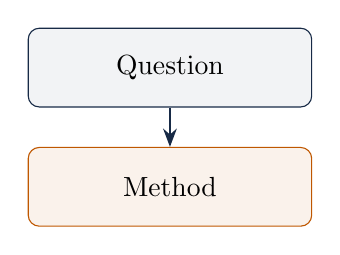
\begin{tikzpicture}[node distance=0.5cm]
\node[draw=LBJnavy,rounded corners,fill=softgray,minimum width=3.6cm,minimum height=1cm] (q) {Question};
\node[draw=UTburnt,rounded corners,fill=UTburnt!8,below=of q,minimum width=3.6cm,minimum height=1cm] (m) {Method};
\draw[-{Stealth},thick,LBJnavy] (q)--(m);
\end{tikzpicture}
\end{columns}
\vfill
\bigquestion{Methods should follow the question, not the other way around.}
\end{frame}

% 4
\begin{frame}{From the world to a dataset}
\centering
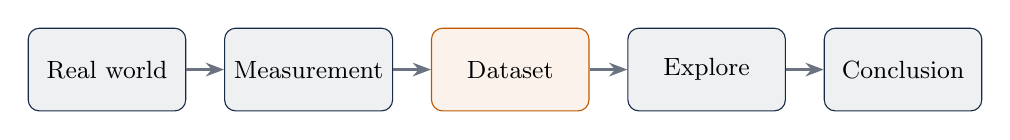
\begin{tikzpicture}[node distance=0.48cm, every node/.style={font=\small}]
\node[draw=LBJnavy,rounded corners,fill=LBJnavy!7,minimum width=2.0cm,minimum height=1.05cm] (world) {Real world};
\node[draw=LBJnavy,rounded corners,fill=LBJnavy!7,right=of world,minimum width=2.0cm,minimum height=1.05cm] (measure) {Measurement};
\node[draw=UTburnt,rounded corners,fill=UTburnt!8,right=of measure,minimum width=2.0cm,minimum height=1.05cm] (data) {Dataset};
\node[draw=LBJnavy,rounded corners,fill=LBJnavy!7,right=of data,minimum width=2.0cm,minimum height=1.05cm] (explore) {Explore};
\node[draw=LBJnavy,rounded corners,fill=LBJnavy!7,right=of explore,minimum width=2.0cm,minimum height=1.05cm] (conclusion) {Conclusion};
\foreach \a/\b in {world/measure,measure/data,data/explore,explore/conclusion}
  \draw[-{Stealth},thick,midgray] (\a)--(\b);
\end{tikzpicture}

\vspace{1.0em}
\begin{block}{A dataset is a simplified representation of the world.}
Every dataset reflects choices about what gets included, what gets measured, how things are defined, and what gets left out.
\end{block}
\end{frame}

% 5
\begin{frame}{The basic building blocks}
\begin{columns}[T,onlytextwidth]
\column{0.42\textwidth}
\begin{itemize}
  \item \alert{Observations / cases}: people, cities, schools, countries, years
  \item \alert{Variables}: characteristics measured for each case
  \item \alert{Values}: what we observe for each variable
\end{itemize}
\column{0.54\textwidth}
\small
\begin{tabular}{lrrl}
\toprule
City & Income & Unemp. & Region \\
\midrule
Austin & 92,000 & 3.4 & South \\
El Paso & 57,000 & 4.6 & South \\
Lubbock & 63,000 & 3.8 & South \\
\bottomrule
\end{tabular}

\vspace{0.8em}
\footnotesize
Rows are observations. Columns are variables. Each cell contains a value.
\end{columns}
\end{frame}

% 6
\begin{frame}{Population and sample}
\begin{columns}[c,onlytextwidth]
\column{0.50\textwidth}
\begin{block}{Population}
Everyone or everything we want to understand.
\end{block}
\begin{block}{Sample}
The cases we actually observe.
\end{block}
\column{0.46\textwidth}
\centering
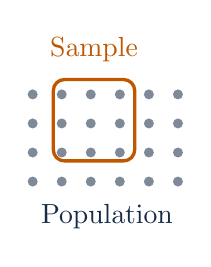
\begin{tikzpicture}[scale=0.82]
\foreach \x in {0,...,5}{
  \foreach \y in {0,...,3}{
    \fill[LBJnavy!55] (0.45*\x,0.45*\y) circle (2.2pt);
  }
}
\draw[UTburnt,very thick,rounded corners] (0.32,0.32) rectangle (1.58,1.58);
\node[align=center,LBJnavy] at (1.15,-0.55) {Population};
\node[align=center,UTburnt] at (0.95,2.05) {Sample};
\end{tikzpicture}
\end{columns}
\vspace{0.5em}
Example: We want to understand \textbf{Texas voters}, but interview \textbf{1,200 Texas voters}.
\end{frame}

% 7
\begin{frame}{Sampling is something we already do}
\begin{columns}[c,onlytextwidth]
\column{0.58\textwidth}
\large
Imagine tasting one spoonful of soup.

\vspace{0.7em}
\begin{itemize}
  \item Spoonful = \alert{sample}
  \item Whole pot = \alert{population}
  \item Deciding whether the pot needs salt = \alert{inference}
\end{itemize}
\column{0.38\textwidth}
\centering
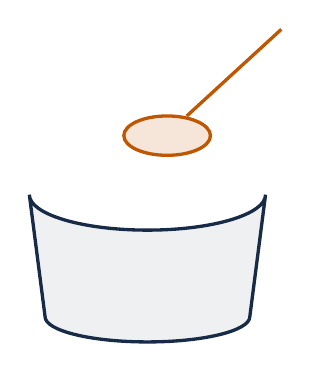
\begin{tikzpicture}
\draw[very thick,LBJnavy,fill=LBJnavy!7] (-1.5,0) arc[start angle=180,end angle=360,x radius=1.5,y radius=0.45] -- (1.3,-1.55) arc[start angle=0,end angle=-180,x radius=1.3,y radius=0.32] -- cycle;
\draw[very thick,UTburnt] (0.5,1.0) -- (1.7,2.1);
\draw[very thick,UTburnt,fill=UTburnt!15] (0.25,0.75) ellipse (0.55 and 0.25);
\end{tikzpicture}
\end{columns}
\vfill
\bigquestion{For an inference to work, the sample needs to tell us something useful about the population.}
\end{frame}

% 8
\begin{frame}[standout]
\Large Measurement: what exactly are we measuring?
\end{frame}

% 9
\begin{frame}{Is Austin becoming less affordable?}
\large
What does \alert{affordable} mean?

\vspace{0.7em}
\begin{columns}[T,onlytextwidth]
\column{0.48\textwidth}
\begin{itemize}
  \item Median rent
  \item Home prices
  \item Rent as a share of income
\end{itemize}
\column{0.48\textwidth}
\begin{itemize}
  \item Cost-burdened households
  \item Homelessness
  \item Income after housing costs
\end{itemize}
\end{columns}
\vfill
\begin{alertblock}{Key point}
Different measures can produce different answers to the same substantive question.
\end{alertblock}
\end{frame}

% 10
\begin{frame}{Variables are representations}
\begin{columns}[T,onlytextwidth]
\column{0.31\textwidth}
\begin{block}{Education}
Years of schooling\\[0.3em]
Highest degree\\[0.3em]
College graduate: yes/no
\end{block}
\column{0.31\textwidth}
\begin{block}{Income}
Individual income\\[0.3em]
Household income\\[0.3em]
Income categories
\end{block}
\column{0.31\textwidth}
\begin{block}{Ideology}
Liberal--conservative\\[0.3em]
Party identification\\[0.3em]
Policy preferences
\end{block}
\end{columns}
\vfill
\bigquestion{There is rarely one inevitable way to measure a concept.}
\end{frame}

% 11
\begin{frame}{Two broad types of variables}
\begin{columns}[T,onlytextwidth]
\column{0.47\textwidth}
\begin{block}{Categorical}
Values represent groups or labels.
\begin{itemize}
  \item Party
  \item Region
  \item Employment status
\end{itemize}
\end{block}
\column{0.47\textwidth}
\begin{block}{Quantitative}
Values represent quantities.
\begin{itemize}
  \item Age
  \item Income
  \item Unemployment rate
\end{itemize}
\end{block}
\end{columns}
\vfill
\alert{Variable type tells us how to summarize and visualize the data.}
\end{frame}

% 12
\begin{frame}[standout]
\Large Exploratory Data Analysis

\vspace{0.5em}
\normalsize
Before we model, we learn what is in the data.
\end{frame}

% 13
\begin{frame}{Start with one variable}
For any variable, ask three questions:

\vspace{0.6em}
\begin{enumerate}
  \item What \alert{values} occur?
  \item How \alert{often} do they occur?
  \item What does the \alert{distribution} look like?
\end{enumerate}

\vfill
\bigquestion{The first goal of EDA is description, not explanation.}
\end{frame}

% 14
\begin{frame}{Categorical variables: count and proportion}
\small
Imagine a hypothetical survey of 100 residents asks whether they support expanding public transit.

\vspace{0.5em}
\begin{columns}[T,onlytextwidth]
\column{0.45\textwidth}
\begin{tabular}{lrr}
\toprule
Response & Count & Proportion \\
\midrule
Support & 52 & 0.52 \\
Oppose & 31 & 0.31 \\
Unsure & 17 & 0.17 \\
\midrule
Total & 100 & 1.00 \\
\bottomrule
\end{tabular}
\column{0.50\textwidth}
\begin{block}{Two useful summaries}
\textbf{Count}: how many observations are in each category.\\[0.6em]
\textbf{Proportion}: the share of observations in each category.
\end{block}
\end{columns}
\vfill
\alert{52 out of 100 = 0.52 = 52\%.}
\end{frame}

% 15
\begin{frame}{Categorical variables: visualize with a bar plot}
\begin{columns}[c,onlytextwidth]
\column{0.58\textwidth}
\centering
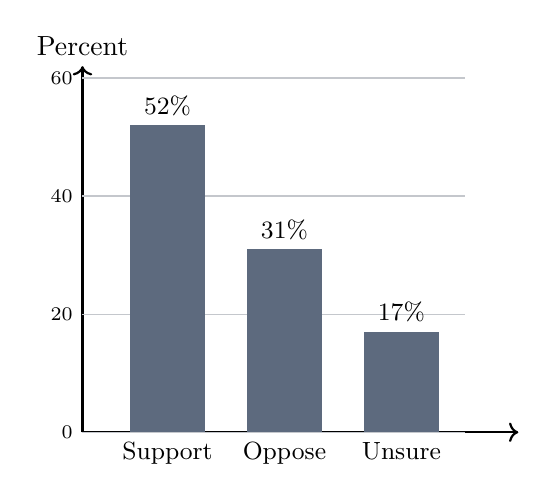
\begin{tikzpicture}[x=1.35cm,y=0.075cm]
\draw[->,thick] (0,0)--(4.1,0);
\draw[->,thick] (0,0)--(0,62) node[above]{Percent};
\foreach \y in {0,20,40,60}{\draw[midgray!40] (0,\y)--(3.6,\y); \node[left,font=\scriptsize] at (0,\y) {\y};}
\fill[LBJnavy!70] (0.45,0) rectangle (1.15,52);
\fill[LBJnavy!70] (1.55,0) rectangle (2.25,31);
\fill[LBJnavy!70] (2.65,0) rectangle (3.35,17);
\node[below,font=\small] at (0.8,0) {Support};
\node[below,font=\small] at (1.9,0) {Oppose};
\node[below,font=\small] at (3.0,0) {Unsure};
\node[above,font=\small] at (0.8,52) {52\%};
\node[above,font=\small] at (1.9,31) {31\%};
\node[above,font=\small] at (3.0,17) {17\%};
\end{tikzpicture}
\column{0.38\textwidth}
\begin{block}{Why a bar plot?}
The height of each bar represents the frequency or proportion in a category.
\end{block}
\vspace{0.5em}
\begin{alertblock}{Your turn}
What is the main pattern in one sentence?
\end{alertblock}
\end{columns}
\end{frame}

% 16
\begin{frame}{Quantitative variables: look at the distribution}
A quantitative variable has many possible values, so counts alone are usually not enough.

\vspace{0.6em}
We want to know:
\begin{itemize}
  \item Where are most observations?
  \item How spread out are they?
  \item Is the distribution symmetric or skewed?
  \item Are there unusual observations?
\end{itemize}
\vfill
\bigquestion{A histogram is often the first place to look.}
\end{frame}

% 17
\begin{frame}{A histogram groups quantitative values}
\begin{columns}[c,onlytextwidth]
\column{0.62\textwidth}
\centering
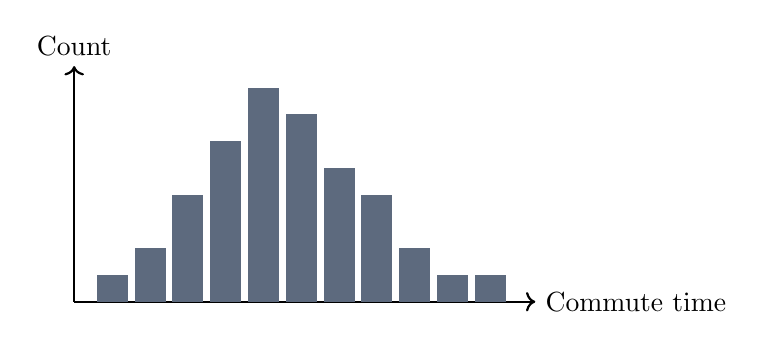
\begin{tikzpicture}[x=0.48cm,y=0.34cm]
\draw[->,thick] (0,0)--(12.2,0) node[right]{Commute time};
\draw[->,thick] (0,0)--(0,8.8) node[above]{Count};
\foreach \x/\h in {0.6/1,1.6/2,2.6/4,3.6/6,4.6/8,5.6/7,6.6/5,7.6/4,8.6/2,9.6/1,10.6/1}{
\fill[LBJnavy!70] (\x,0) rectangle +(0.82,\h);
}
\end{tikzpicture}
\column{0.34\textwidth}
\begin{block}{Read the shape}
Most observations are clustered in the middle, with fewer long commutes.
\end{block}
\end{columns}
\vfill
\alert{The exact bars depend on how the values are grouped into bins.}
\end{frame}

% 18
\begin{frame}{Something looks strange}
\begin{columns}[c,onlytextwidth]
\column{0.52\textwidth}
Imagine a class survey asks:

\vspace{0.5em}
\begin{center}
\textit{``How old were you when you had your first kiss?''}
\end{center}

Most answers fall between 12 and 20, but several students report ages 0--3.
\column{0.44\textwidth}
\centering
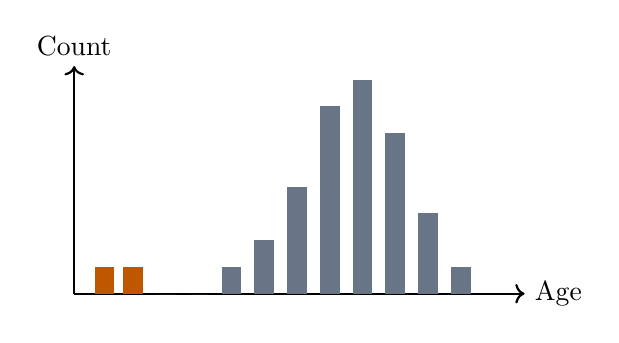
\begin{tikzpicture}[x=0.52cm,y=0.34cm]
\draw[->,thick] (0,0)--(11,0) node[right]{Age};
\draw[->,thick] (0,0)--(0,8.5) node[above]{Count};
\foreach \x/\h in {0.5/1,1.2/1,2.0/0,2.8/0,3.6/1,4.4/2,5.2/4,6.0/7,6.8/8,7.6/6,8.4/3,9.2/1}{\fill[LBJnavy!65] (\x,0) rectangle +(0.48,\h);}
\fill[UTburnt] (0.5,0) rectangle +(0.48,1);
\fill[UTburnt] (1.2,0) rectangle +(0.48,1);
\end{tikzpicture}
\end{columns}
\vfill
\begin{alertblock}{What might be going on?}
The question may be ambiguous: a romantic kiss, or any kiss?
\end{alertblock}
\end{frame}

% 19
\begin{frame}{Measuring the center: the mean}
The \alert{mean} is the arithmetic average.

\vspace{0.6em}
\[
\bar{x}=\frac{x_1+x_2+\cdots+x_n}{n}
\]

\vspace{0.4em}
Example commute times, in minutes:

\begin{center}
10, 12, 15, 18, 20, 22, 25, 27, 30, 120
\end{center}

\vfill
\begin{alertblock}{Mean commute time}
\centering
29.9 minutes
\end{alertblock}
\end{frame}

% 20
\begin{frame}{Measuring the center: the median}
The \alert{median} is the middle value after ordering the observations.

\vspace{0.6em}
\begin{center}
10, 12, 15, 18, \alert{20, 22}, 25, 27, 30, 120
\end{center}

With an even number of observations, take the average of the two middle values.

\[
\text{Median}=\frac{20+22}{2}=21
\]

\vfill
\bigquestion{Why is the mean 29.9 but the median only 21?}
\end{frame}

% 21
\begin{frame}{Mean or median? Look at the distribution}
\begin{columns}[T,onlytextwidth]
\column{0.47\textwidth}
\begin{block}{Mean}
Uses every value.\\[0.4em]
Sensitive to extreme observations.\\[0.4em]
Often useful for roughly symmetric distributions.
\end{block}
\column{0.47\textwidth}
\begin{block}{Median}
Uses the ordering of values.\\[0.4em]
Resistant to extreme observations.\\[0.4em]
Often useful for skewed distributions.
\end{block}
\end{columns}
\vfill
\alert{The ``best'' summary depends on what the distribution looks like.}
\end{frame}

% 22
\begin{frame}{Center is not enough: we also need spread}
Two neighborhoods can have the same average commute but very different experiences.

\vspace{0.6em}
\begin{columns}[T,onlytextwidth]
\column{0.47\textwidth}
\begin{block}{Neighborhood A}
24, 25, 25, 26, 25\\[0.5em]
Mean = 25
\end{block}
\column{0.47\textwidth}
\begin{block}{Neighborhood B}
5, 15, 25, 35, 45\\[0.5em]
Mean = 25
\end{block}
\end{columns}
\vfill
\bigquestion{Same center. Very different spread.}
\end{frame}

% 23
\begin{frame}{Two simple measures of spread}
\begin{columns}[T,onlytextwidth]
\column{0.47\textwidth}
\begin{block}{Range}
Maximum $-$ minimum

\vspace{0.4em}
For our commute example:
\[
120-10=110
\]
\end{block}
\column{0.47\textwidth}
\begin{block}{Interquartile range (IQR)}
Spread of the middle 50\% of observations.

\vspace{0.4em}
\[
IQR=Q_3-Q_1
\]
\end{block}
\end{columns}
\vfill
\alert{Like the median, the IQR is less sensitive to extreme values.}
\end{frame}

% 24
\begin{frame}{Standard deviation: a preview}
The \alert{standard deviation} summarizes how far observations typically fall from the mean.

\vspace{0.7em}
\begin{columns}[c,onlytextwidth]
\column{0.58\textwidth}
\begin{itemize}
  \item Small SD: values cluster near the mean.
  \item Large SD: values are more dispersed.
  \item It is expressed in the same units as the variable.
\end{itemize}
\column{0.38\textwidth}
\centering
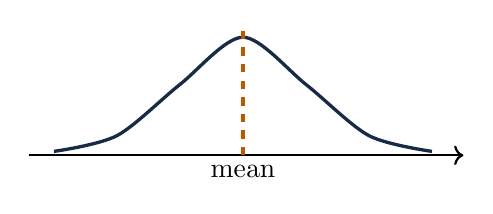
\begin{tikzpicture}[x=0.8cm,y=0.5cm]
\draw[->,thick] (-3.4,0)--(3.5,0);
\draw[LBJnavy,very thick] plot[smooth] coordinates {(-3,0.1)(-2,0.5)(-1,1.8)(0,3)(1,1.8)(2,0.5)(3,0.1)};
\draw[UTburnt,very thick,dashed] (0,0)--(0,3.2);
\node[below] at (0,0) {mean};
\end{tikzpicture}
\end{columns}
\vfill
\footnotesize We will develop the standard deviation more carefully when we study distributions and probability.
\end{frame}

% 25
\begin{frame}{Match the variable to the summary}
\small
\begin{center}
\begin{tabular}{>{\raggedright\arraybackslash}p{0.23\textwidth} >{\raggedright\arraybackslash}p{0.31\textwidth} >{\raggedright\arraybackslash}p{0.31\textwidth}}
\toprule
\textbf{Variable} & \textbf{Useful numerical summary} & \textbf{Useful visualization} \\
\midrule
Categorical & Count, proportion / percentage & Bar plot \\
\addlinespace
Quantitative & Mean or median + measure of spread & Histogram, boxplot \\
\bottomrule
\end{tabular}
\end{center}

\vspace{0.9em}
\begin{alertblock}{A good habit}
Do not report a mean without first looking at the distribution that produced it.
\end{alertblock}
\end{frame}

% 26
\begin{frame}{Before you trust a summary, inspect the data}
\begin{columns}[T,onlytextwidth]
\column{0.48\textwidth}
\begin{block}{Look for}
\begin{itemize}
  \item Missing values
  \item Impossible values
  \item Unexpected categories
  \item Extreme observations
\end{itemize}
\end{block}
\column{0.48\textwidth}
\begin{block}{Ask why}
A strange value could be:
\begin{itemize}
  \item real,
  \item a data-entry error,
  \item a coding problem,
  \item a measurement problem.
\end{itemize}
\end{block}
\end{columns}
\vfill
\bigquestion{Investigate first. Do not automatically delete unusual observations.}
\end{frame}

% 27
\begin{frame}{What can the evidence support?}
\begin{columns}[T,onlytextwidth]
\column{0.31\textwidth}
\begin{block}{Description}
\textbf{What is happening?}\\[0.5em]
What percentage of Texans lack health insurance?
\end{block}
\column{0.31\textwidth}
\begin{block}{Association}
\textbf{Are two things related?}\\[0.5em]
Is income related to insurance coverage?
\end{block}
\column{0.31\textwidth}
\begin{block}{Causation}
\textbf{Does X change Y?}\\[0.5em]
Does expanding Medicaid increase coverage?
\end{block}
\end{columns}
\vfill
\alert{Today we focused on description. Association and causation require additional tools.}
\end{frame}

% 28
\begin{frame}{The workflow we start this week}
\centering
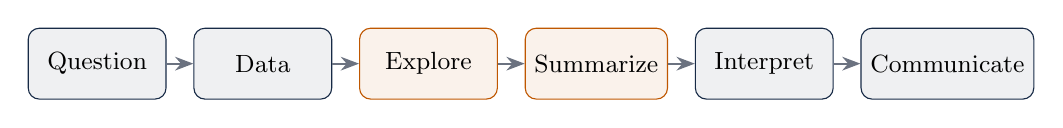
\begin{tikzpicture}[node distance=0.34cm,every node/.style={font=\small}]
\node[draw=LBJnavy,rounded corners,fill=LBJnavy!7,minimum width=1.75cm,minimum height=0.9cm] (q) {Question};
\node[draw=LBJnavy,rounded corners,fill=LBJnavy!7,right=of q,minimum width=1.75cm,minimum height=0.9cm] (d) {Data};
\node[draw=UTburnt,rounded corners,fill=UTburnt!8,right=of d,minimum width=1.75cm,minimum height=0.9cm] (e) {Explore};
\node[draw=UTburnt,rounded corners,fill=UTburnt!8,right=of e,minimum width=1.75cm,minimum height=0.9cm] (a) {Summarize};
\node[draw=LBJnavy,rounded corners,fill=LBJnavy!7,right=of a,minimum width=1.75cm,minimum height=0.9cm] (i) {Interpret};
\node[draw=LBJnavy,rounded corners,fill=LBJnavy!7,right=of i,minimum width=1.75cm,minimum height=0.9cm] (c) {Communicate};
\foreach \x/\y in {q/d,d/e,e/a,a/i,i/c}{\draw[-{Stealth},thick,midgray] (\x)--(\y);}
\end{tikzpicture}

\vspace{1.2em}
\begin{block}{Wednesday in R}
We will identify variable types, inspect data, calculate counts/proportions and simple numerical summaries, and create a visualization in a reproducible document.
\end{block}
\vfill
\bigquestion{If I give you a variable, how should you summarize and visualize it?}
\end{frame}

\end{document}
